%SOP Template 
% Version 02 Added revision date
% Version 03 Added TOC and acknowledgements
%           New SOP3_alpha.cls


\documentclass[12pt]{../SOP3_alpha}

\usepackage[english]{babel}
\usepackage{blindtext}
\usepackage{lipsum}

\title{Using Everyday Lab Equipment }
\date{8/10/2016}
\author{Reseacher Name}
\approved{TBD}
\ReviseDate{8/10/16}
\SOPno{09 v.01}

\usepackage{Sweave}
\begin{document}
\Sconcordance{concordance:Balance_Pippite_Glassware_v01.tex:Balance_Pippite_Glassware_v01.Rnw:%
1 19 1 1 0 76 1}


\maketitle 
Using Everyday Lab Equipment 

\section{Scope and Application}

\NP The scope of this SOP is  to train researchers to learn and follow the basic protocol of using, cleaning, and operating everyday lab equipment, which includes, the micropipette, glassware equipment, measuring balances, the Vortex, and other marginal lab tools that will be further specified. 

\NP The applications of this SOP are for any basic lab setting for students conducting experiments and/or learning new lab procedures.

\section{Summary of Method}

\NP 

\tableofcontents

\newpage

\section{Acknowledgements}

\section{Definitions}

\NP Term1:


\section{Health and Safety}

\NP Describe the risk...


\subsection*{Safety and Personnnel Protective Equipment}


\section{Personnel \& Training Responsibilities}

\NP Researchers training is required before this the procedures in this method can be used... 

\NP Researchers using this SOP should be trained for the following SOPs:

\begin{itemize}
  \item SOP01 Laboratory Safety
  \item SOP02 Field Safety
\end{itemize} 

\section{Apparati}

\NP Pipetman (ranging from 2-1000microliters)
\section {What is a Micropipette?}
Micropipettes are used to transfer small amounts (< 1 ml) of liquids. The scales on micropipettes are in microliters (1000 µl = 1 ml). These are very expensive, delicate instruments so be very careful during use. The sizes of the micropipettes can be identified via the number on the round button on the plunger; this value is the maximum volume in microliters that can be transferred with that size pipette. The following is an illustration of a micropipette:
\begin{figure} [H!]
\caption{The Pipetman}
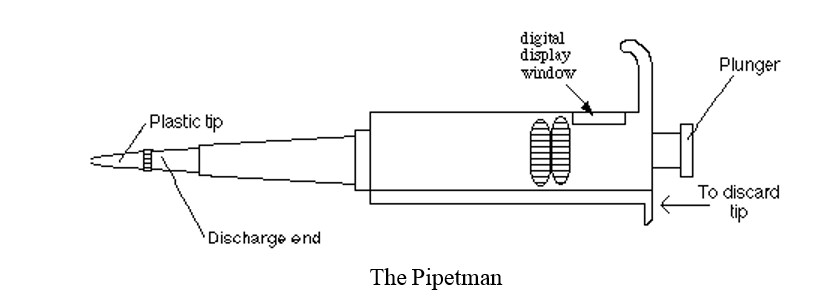
\includegraphics{pipetman.jpg}
\end{figure}

\section {How to Use a Micropipette}
\begin{enumerate}
  \item NEVER exceed the upper or lower limits of these pipettes.
The limits are:  P10: 1.0 - 10.0 µl; P20: 2.0 - 20.0 µl; P200: 20 - 200 µl; P1000: 200 - 1000 µl  
Look at the front face of the pipet and you will see a window with three digits inside. The diagram below shows the MAXIMUM value that can or should be dialed in on each size pipet. To exceed these values will put the pipet out of calibration. Beside each "window" below is the numbers place it represents. (figure \ref{fig:pipetman})
\begin{figure} [H!]
\caption{Pipetman Window}
\label{fig:pipetman}
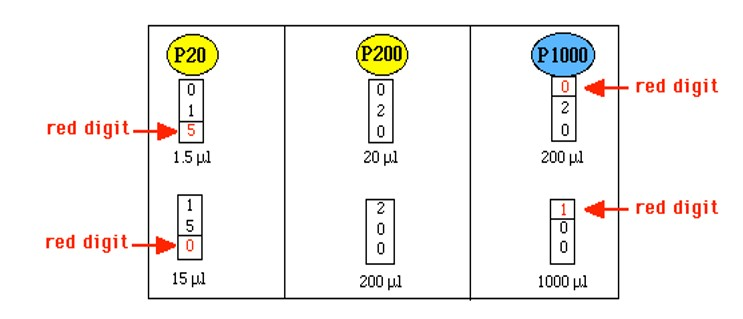
\includegraphics{pipetman2.jpg}
\end{figure}
\begin{itemize}
  \item RULE OF THUMB: Always select the SMALLEST size pipette that will handle the volume you wish to move to achieve the greatest accuracy. Accuracy decreases as you use unnecessarily large pipets for small volumes.   
\end{itemize}
\item Set the desired volume by turning the centrally located rings clockwise to increase volume or counterclockwise to decrease volume.  
\item Load a sterile tip. Use the appropriate tips for each micropipette as designated by the labels of the box, and by confirming with the lab instructor. 
\item 5.	 Load the sample. 
\begin{itemize}
  \item The plunger will stop at two different positions when it is depressed. Push the plunger down slowly to the point of first resistance: this is the load volume. Because this first stopping point is dependent on the volume that is being transferred, the distance you have to push the plunger to reach the point of initial resistance will change depending on the volume being pipetted. 
  \item While holding the plunger at the load volume set point, put the tip into the solution so that it is immersed just enough to cover the end (3-4 mm), not as deep as possible. 
  \item Slowly release the plunger to draw up the liquid making sure to keep the tip immersed. \textbf{NOTE:} If the solution you are pipetting is viscous, allow the pipet tip to fill to final volume before removing it from solution to avoid the presence of bubbles in the plastic tip, which will result in an inaccurate volume.
  \item Visually inspect the load to make sure it is correct - there should be no air space in the distal end tip.
\end{itemize}

\begin{figure} [H!]
\caption{Loading Sample}
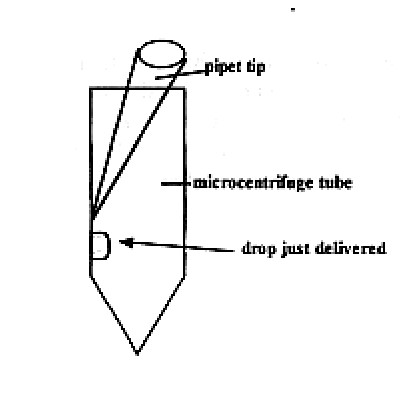
\includegraphics{pipetman3.jpg}
\end{figure}

\item Deliver the sample. The second stopping point can be found when the plunger is depressed beyond the initial resistance until it is in contact with the body of the pipette. This second stopping point is used for the complete discharging of solutions from the plastic tip. You should not reach this second stop when drawing liquid into the pipette, only when expelling the last drop.   
\item Discharge the tip. While holding the tip over an appropriate waste receptacle, press the discharge slider on the back of the grip.     

\end{enumerate}
\section{Things to Keep in Mind}
\begin{itemize}
  \item Do not hesitate to ask the lab instructor questions about the pipetting protocol and measures to avoid contamination 
\item Never point a pipette up. This may cause liquid to run down into the pipette destroying it
\item When withdrawing liquids with the pipette, always release the plunger slowly. This prevents liquid from rushing into the end of the pipette and clogging it up.  This is especially important with large volume pipettes 
\item Be sure you use the proper size tip for each pipette. 
\item Always use a new tip for each different liquid.
\item Use the correct pipette for the volume that is to be dispensed. Going below or above the range of the micropipette may damage the instrument.      

\end{itemize}


\NP Vortex Mixer
\NP Glassware
\NP Balances 



\section{QC/QA Criteria}

\section{References}

\NP APHA, AWWA. WEF. (2012) Standard Methods for examination of water and wastewater. 22nd American Public Health Association (Eds.). Washington. 1360 pp. (2014).

\end{document}
